\chapter{Methodology}
\label{chap:methodology}

\section{Baseline: Classical 3D Gaussian Splatting}
\label{sec:baseline_3dgs}

All extensions developed in this thesis are evaluated against a \emph{classical} 3D Gaussian Splatting baseline implemented as Nerfstudio's \textbf{Splatfacto} method (\texttt{splatfacto}), with default configuration \texttt{loss=rgb} and no depth term, semantic masks, or B\'ezier reparameterization. Unless stated otherwise, experiments use the same data preparation pipeline (COLMAP $\rightarrow$ \filepath{transforms.json}) and the same \texttt{FullImageDataManager}. Baseline and depth-supervised runs retain upstream Splatfacto's adaptive clone/split/prune densification \cite{kerbl2023gaussian,tancik2023nerfstudio}; B\'ezier runs disable densification and optimize a fixed $(N_u,N_v)$ lattice on each patch instead (Section~\ref{subsec:bezier_pipeline}).

\subsection{Photometric Loss}
\label{subsec:baseline_photometric}

Baseline training optimizes only image consistency. For each sampled training camera $V$ with ground-truth RGB $I_{\mathrm{gt}}$, Splatfacto rasterizes the current Gaussian set and obtains $\hat{I}$. The objective matches the formulation in Section~2.3.5:
\begin{align}
\mathcal{L}_{\mathrm{rgb}} &= (1-\lambda)\,\mathcal{L}_{1}+\lambda\,\mathcal{L}_{\text{D-SSIM}}, \\
\mathcal{L}_{1} &= \|\hat{I}-I_{\mathrm{gt}}\|_{1}, \\
\mathcal{L}_{\text{D-SSIM}} &= \frac{1-\mathrm{SSIM}(\hat{I},I_{\mathrm{gt}})}{2},
\label{eq:baseline_photometric}
\end{align}
with $\lambda=0.2$ (\code{ssim\_lambda} in the default configuration). Gradients flow back through the differentiable \code{gsplat} rasterizer to update Gaussian means, covariances (via quaternion and log-scale parameters), opacities, and spherical-harmonic color coefficients. Camera poses are optionally refined by the standard Nerfstudio camera optimizer; no auxiliary geometric loss is active in this mode.

This photometric-only setting defines the reference against which depth supervision (Section~\ref{sec:depth_supervised}) and B\'ezier-based structural changes (Section~\ref{sec:bezier_structural}) are motivated; B\'ezier outcomes are evaluated in Chapter~\ref{chap:results}.

\begin{figure}[H]
    \centering
    
\includegraphics[width=0.92\textwidth]{{images/methodology/3d_gaussian viewer_output.png}}
    \caption{Baseline Splatfacto checkpoint exported and inspected in \textbf{SuperSplat} \cite{supersplat2024}, a web-based 3DGS viewer (\url{https://superspl.at/}).
    \textbf{Top left:} scene render with semi-transparent Gaussian splats (unstructured early or diagnostic view).
    \textbf{Top right:} shaded RGB rendering of the reconstructed scene.
    \textbf{Bottom left:} Gaussian \emph{centers} visualized as point sprites (``puntini'') overlaid on the render.
    \textbf{Bottom right:} anisotropic Gaussian \emph{ellipsoids} drawn with wireframe contours, showing the extent and orientation of each primitive.}
    \label{fig:baseline_viewer_outputs}
\end{figure}

\subsection{Expected Depth Estimation}
\label{subsec:baseline_expected_depth}

Although the baseline \emph{loss} does not supervise depth, rendered depth maps are still useful for analysis, export, and as the prediction target when \texttt{loss=depth} is enabled later. Following the volume-rendering viewpoint in Section~2.4.1, each pixel corresponds to a discrete set of front-to-back contributions with compositing weights $w_i=\alpha_i T_i$. The \emph{expected depth} along the viewing direction is
\begin{equation}
d^{\mathrm{exp}}_{x,y}=\frac{\sum_i z_i\,w_i}{\sum_i w_i},
\label{eq:baseline_depth_expected}
\end{equation}
where $z_i$ is the depth coordinate associated with Gaussian $i$ (in the implementation, camera $z$-depth in meters).

In Splatfacto, this quantity is obtained from the \texttt{gsplat} rasterizer by setting \texttt{render\_mode="RGB+ED"}: the fourth channel of the render buffer is the alpha-weighted expected depth, masked where accumulation $\alpha$ is zero. During baseline training (\texttt{loss=rgb}, \texttt{output\_depth\_during\_training=False}), depth is \emph{not} computed on every step to save memory; it is produced at evaluation time and can be exported at the end of training (\texttt{export\_outputs}).

\begin{figure}[H]
    \centering
    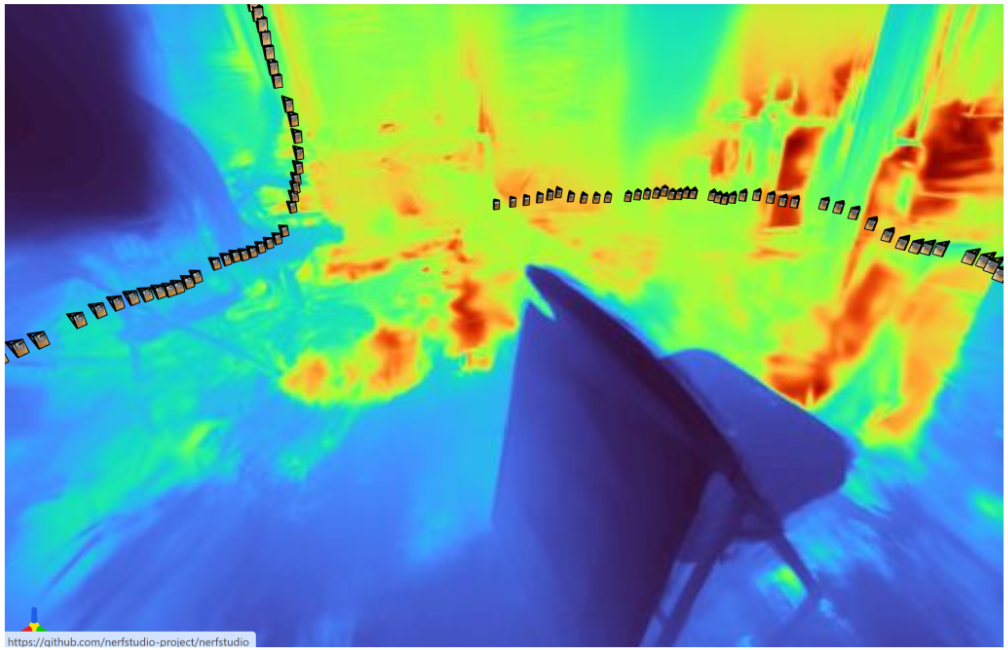
\includegraphics[width=0.85\textwidth]{images/methodology/3dgaussian_expected_depth_out.png}
    \caption{Expected depth $d^{\mathrm{exp}}$ from the baseline rasterizer (\texttt{RGB+ED}), visualized in the Nerfstudio viewer as a false-color map together with the training camera poses. Closer surfaces appear in cooler colors and farther ones in warmer colors (default \texttt{turbo} colormap); background and low-accumulation pixels remain dark. This map is used later as the rendered-depth target when \texttt{loss=depth} is enabled (Section~\ref{sec:depth_supervised}).}
    \label{fig:baseline_expected_depth}
\end{figure}

The codebase also exposes an optional \textbf{ellipsoid depth} mode (\texttt{depth\_mode="ellipsoid"}), which returns the depth of the first ray--ellipsoid hit above a Mahalanobis threshold; it was implemented for diagnostic comparison but is not used in any experiment reported here.

\subsection{Observed Geometric Limitations}
\label{subsec:baseline_limitations}

Empirically, baseline models trained with $\mathcal{L}_{\mathrm{rgb}}$ alone often reach high PSNR/SSIM while yielding unstable explicit geometry. As discussed in Section~2.3.7, 3DGS optimizes photometric consistency rather than explicit surface regularity: several Gaussians can overlap along the same viewing ray, expected depth can look locally sharp while the global depth field stays compressed or inconsistent across views, and exports (point clouds, meshes) remain noisy in low-texture, occluded, or poorly observed regions (Figures~\ref{fig:baseline_viewer_outputs} and~\ref{fig:baseline_expected_depth}).

Detached high-opacity primitives---\emph{floaters} (Figure~\ref{fig:floaters_example})---are one visible symptom of this mismatch, especially behind reflective or transparent surfaces and along depth discontinuities, but they are neither necessary nor sufficient to explain poor geometry on their own. The same photometric objective also encourages broader anisotropic blobs and depth stratification that need not correspond to a single physical surface.

High photometric scores are therefore a weak indicator of metric geometry on their own. The rest of the chapter contrasts two complementary responses against this baseline. Section~\ref{sec:depth_supervised} keeps the classical Gaussian cloud and adds a global depth prior (DA3) on the rendered expected depth $d^{\mathrm{exp}}$, biasing layout toward a dense metric field while leaving densification and free primitive placement unchanged. Section~\ref{sec:bezier_structural} takes a different route: semantically isolated object seeds (Grounding DINO and SAM~2) are fitted with B\'ezier patches and Gaussians are seeded on a fixed $(u,v)$ lattice, trading full-scene flexibility for an explicit, exportable surface on the target object.

\section{Depth-Supervised Optimization}
\label{sec:depth_supervised}

The second methodological extension replaces the photometric $L_1$ term of Section~\ref{sec:baseline_3dgs} with a depth-consistency term, while keeping the same Gaussian parameterization, densification schedule, and COLMAP-based initialization. Training is activated by setting \texttt{loss=depth} in \texttt{SplatfactoModelConfig}; the predicted depth is the rasterizer expected depth $d^{\mathrm{exp}}$ (Eq.~\eqref{eq:baseline_depth_expected}), and the target is a monocular \emph{metric} prior from Depth Anything~3 (DA3METRIC-LARGE, Section~2.4.3).

\subsection{Ground Truth Depth Generation}
\label{subsec:da3_gt_depth}

Unlike relative-depth models (e.g.\ Depth Anything~V2 \cite{yang2024depthanythingv2}), which require per-image scale--shift alignment before supervision, this work uses the \textbf{DA3 metric} checkpoint \codeid{depth-anything/da3metric-large}. For each training RGB image $I$ with known focal length $f$ in pixels (from COLMAP intrinsics), DA3 returns a network output $\hat{d}_{\mathrm{net}}$ that is converted to metric camera depth in meters by
\begin{equation}
d_{\mathrm{DA3}} = \frac{f\,\hat{d}_{\mathrm{net}}}{300},
\label{eq:da3_metric}
\end{equation}
following the model-card convention implemented in \filepath{nerfstudio/models/da3\_depth.py}. Depth is inferred \emph{independently per view}; multi-view cross-attention and ray-map outputs of the full DA3 framework are not used at training time (Section~2.4.3).

\paragraph{Preprocessing and caching.}
Ground-truth depth maps can be materialized offline during dataset conversion (\code{ns-process-data images --use-da3-depth}), which writes 16-bit PNGs under \filepath{depth/} and registers them in \filepath{transforms.json}. At training time, Splatfacto first reads \code{batch["depth\_image"]} when present; otherwise it falls back to on-the-fly DA3 inference with an in-memory (and optional on-disk) cache keyed by camera index.

\begin{lstlisting}[caption={Metric conversion in \code{DA3MetricDepthEstimator.infer\_metric\_depth} (\filepath{da3\_depth.py}).},label={lst:da3_metric}]
pred = model.inference([img_uint8]).depth[0]   # network output
metric = (pred * focal_px) / 300.0             # meters, per DA3METRIC-LARGE
\end{lstlisting}

\begin{figure}[H]
    \centering
    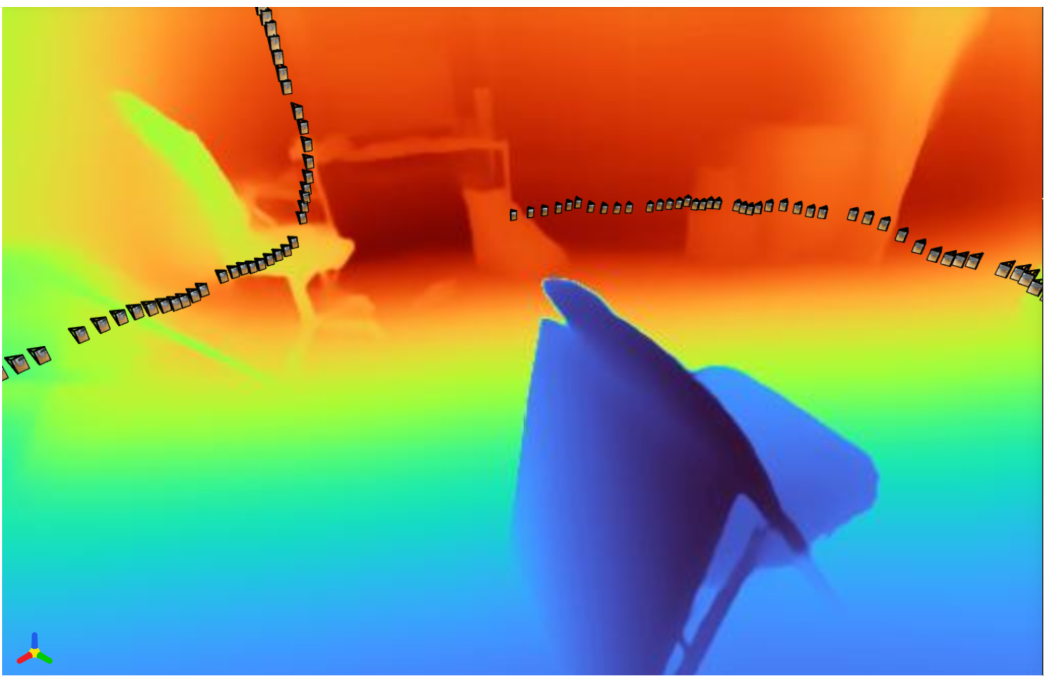
\includegraphics[width=0.75\textwidth]{images/methodology/dav3_output.png}
    \caption{Example DA3 metric depth target ($d_{\mathrm{DA3}}$) visualized in the Nerfstudio viewer for one training view. Warmer colors denote larger camera $z$-depth.}
    \label{fig:da3_depth_target}
\end{figure}

\subsection{Depth Loss Formulation}
\label{subsec:depth_loss}

When \texttt{loss=depth}, the main training objective supervises rendered depth instead of RGB. Let $d^{\mathrm{exp}}$ be the expected depth from \texttt{render\_mode="RGB+ED"} and $d_{\mathrm{DA3}}$ the pseudo ground truth for the same view (resampled to the current training resolution). The primary loss is
\begin{equation}
\mathcal{L}_{\mathrm{depth}} = \frac{1}{|\Omega|}\sum_{(x,y)\in\Omega}\left|d^{\mathrm{exp}}_{x,y}-d_{\mathrm{DA3},x,y}\right|,
\label{eq:depth_loss}
\end{equation}
where $\Omega$ is the set of valid pixels (optionally restricted by a segmentation mask). Importantly, the D-SSIM term on RGB is \textbf{not} added in this mode: appearance is no longer directly optimized at each step, although RGB is still rendered for logging and evaluation.

\begin{lstlisting}[caption={Depth branch in \texttt{SplatfactoModel.get\_loss\_dict} (\filepath{splatfacto.py}).},label={lst:depth_loss_code}]
if self.config.loss == "depth":
    pred_depth = outputs["depth"]          # RGB+ED expected depth
    gt_depth = batch["depth_image"]        # or DA3 on-the-fly
    Ll1 = torch.abs(gt_depth - pred_depth).mean()
    loss_dict = {"main_loss": Ll1, ...}   # no SSIM term
else:
    Ll1 = torch.abs(gt_img - pred_img).mean()
    simloss = 1 - self.ssim(gt_img, pred_img)
    loss_dict = {"main_loss": (1-lambda)*Ll1 + lambda*simloss, ...}
\end{lstlisting}

Gradients therefore flow primarily into Gaussian positions, scales, and opacities (the parameters that influence $d^{\mathrm{exp}}$), rather than into spherical-harmonic color coefficients.

\subsection{Joint Optimization Strategy}
\label{subsec:depth_joint_opt}

Apart from the swapped $L_1$ term, the optimization loop is unchanged: adaptive clone/split/prune, optional camera-pose refinement, and the same learning-rate schedules as the RGB baseline. Expected depth is enabled during training (\texttt{output\_depth\_during\_training} implicitly via \texttt{loss=depth}) so that $\mathcal{L}_{\mathrm{depth}}$ can be evaluated every iteration.

\paragraph{Role of COLMAP color initialization.}
A key observation, relevant when comparing RGB and depth renders, is that Gaussian \emph{colors} are initialized from COLMAP tie points, which carry per-point RGB estimates in addition to 3D position. In \texttt{SplatfactoModel.populate\_modules}, the DC spherical-harmonic coefficients are set from these colors via \texttt{RGB2SH} before the first training step. As a result, the scene is already chromatically recognizable at iteration zero, even though $\mathcal{L}_{\mathrm{depth}}$ does not update appearance. This explains why novel-view RGB can look broadly similar between \texttt{loss=rgb} and \texttt{loss=depth} experiments, despite very different geometric gradients.

\begin{lstlisting}[caption={Color initialization from COLMAP seed points (\filepath{splatfacto.py}).},label={lst:colmap_color_init}]
shs[:, 0, :3] = RGB2SH(seed_rgb / 255)   # seed_rgb from sparse SfM points
features_dc = torch.nn.Parameter(shs[:, 0, :])
\end{lstlisting}

\subsection{Qualitative Trade-offs: RGB vs.\ Depth Loss}
\label{subsec:depth_rgb_tradeoff}

Although final RGB images can appear similar because of shared initialization, the \emph{depth maps} and \emph{internal Gaussian layouts} differ markedly between the two loss modes. Figures~\ref{fig:rgb_depth_render_compare} and~\ref{fig:rgb_depth_depth_compare} summarize the behavior observed on the same indoor scene (chair and poster).

\paragraph{Training with $\mathcal{L}_{\mathrm{rgb}}$ (photometric loss).}
The photometric objective forces the model to explain local intensity patterns, object contours, and high-frequency texture. To reduce $\mathcal{L}_{\mathrm{rgb}}$, Gaussians often stratify along the viewing direction in front of salient structures: multiple semi-transparent layers stack in depth and collectively contribute to both color and $d^{\mathrm{exp}}$. On the foreground object, this can yield depth estimates that look locally sharp; however, the background exhibits higher speckle noise, a compressed global depth range, and reduced multi-view coherence. Figure~\ref{fig:supersplat_rgb_vs_depth} (left) shows this effect in SuperSplat: dense overlapping ellipsoids with visible contours along viewing rays.

\paragraph{Training with $\mathcal{L}_{\mathrm{depth}}$ (depth loss).}
Here the optimizer is driven mainly by a \emph{global} depth field. Gaussians tend to collapse their extent along the ray direction and concentrate around a representative depth, producing smoother background depth closer to the DA3 prior range, but at the cost of local geometric ambiguity on the object (blurred structure, missing thin parts, and depth bleeding at discontinuities). In other words, depth supervision improves global depth coherence while being less constrained on fine local geometry; the opposite trade-off of photometric training.

\begin{figure}[H]
    \centering
    \begin{subfigure}[b]{0.48\textwidth}
        \centering
        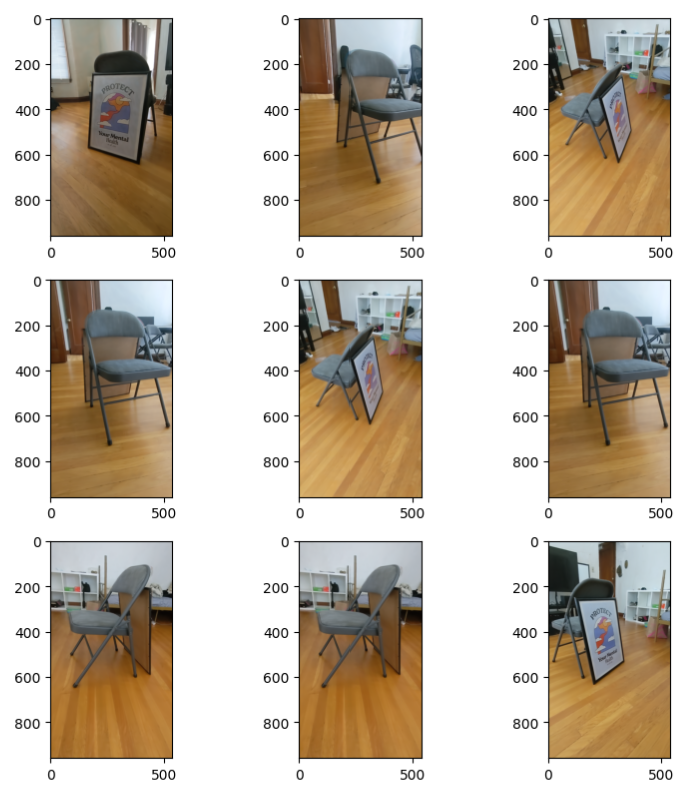
\includegraphics[width=\textwidth]{images/methodology/loss_classica_render_rgb.png}
        \caption{\texttt{loss=rgb}}
        \label{fig:rgb_loss_render}
    \end{subfigure}
    \hfill
    \begin{subfigure}[b]{0.48\textwidth}
        \centering
        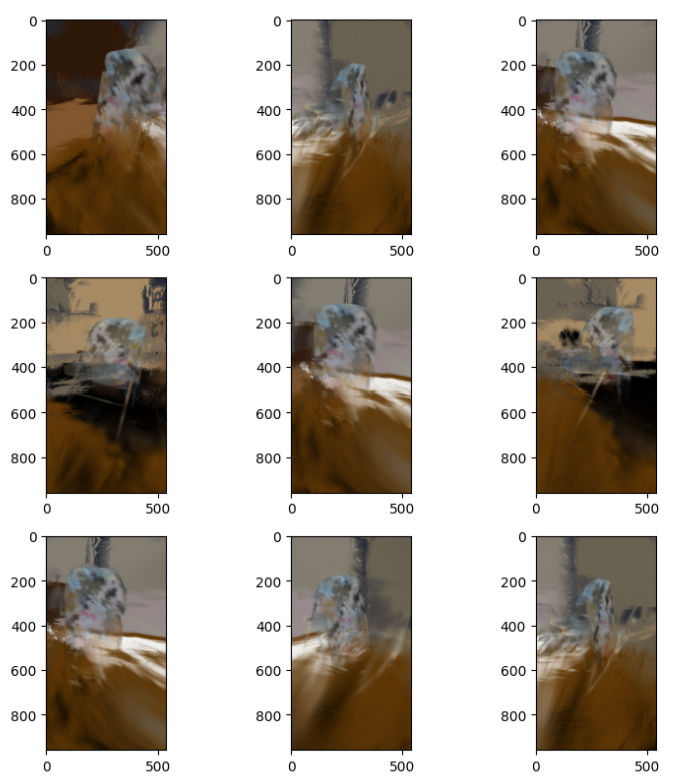
\includegraphics[width=\textwidth]{images/methodology/loss_depth_render_rgb.png}
        \caption{\texttt{loss=depth}}
        \label{fig:depth_loss_render}
    \end{subfigure}
    \caption{Rendered RGB on held-out views after training with photometric loss (left) versus depth loss (right). Overall color layout is similar because both runs share COLMAP color initialization, even though only the left model optimizes appearance.}
    \label{fig:rgb_depth_render_compare}
\end{figure}

\begin{figure}[H]
    \centering
    \begin{subfigure}[b]{0.48\textwidth}
        \centering
        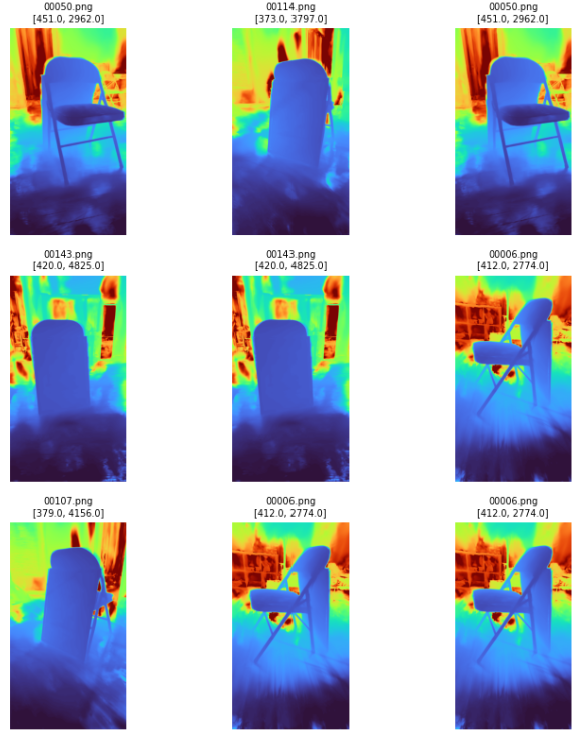
\includegraphics[width=\textwidth]{images/methodology/loss_classica_expected_depth.png}
        \caption{\texttt{loss=rgb}}
        \label{fig:rgb_loss_depthmap}
    \end{subfigure}
    \hfill
    \begin{subfigure}[b]{0.48\textwidth}
        \centering
        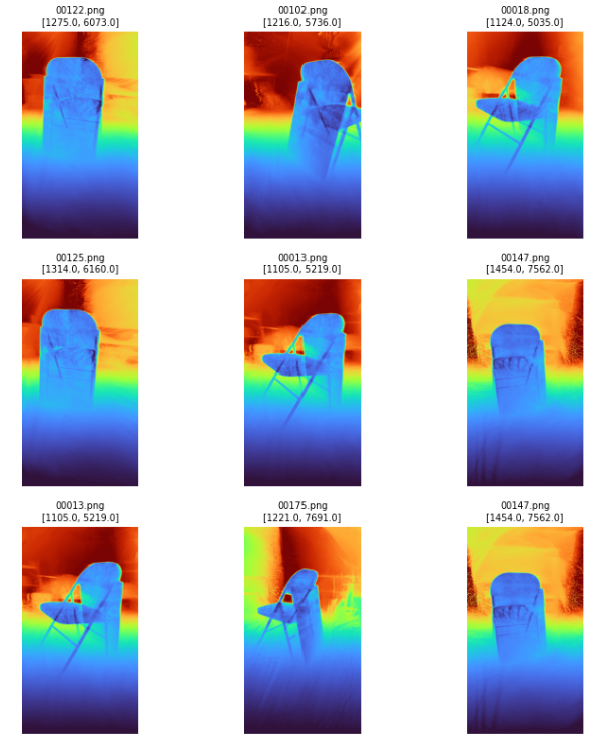
\includegraphics[width=\textwidth]{images/methodology/loss_depth_expected_depth.png}
        \caption{\texttt{loss=depth}}
        \label{fig:depth_loss_depthmap}
    \end{subfigure}
    \caption{Exported expected depth $d^{\mathrm{exp}}$ for the same scene: photometric training (left) shows sharper object silhouettes but noisier background and a narrower effective depth range; depth training (right) yields smoother background depth closer to the DA3 prior, with softer object detail.}
    \label{fig:rgb_depth_depth_compare}
\end{figure}

\begin{figure}[H]
    \centering
    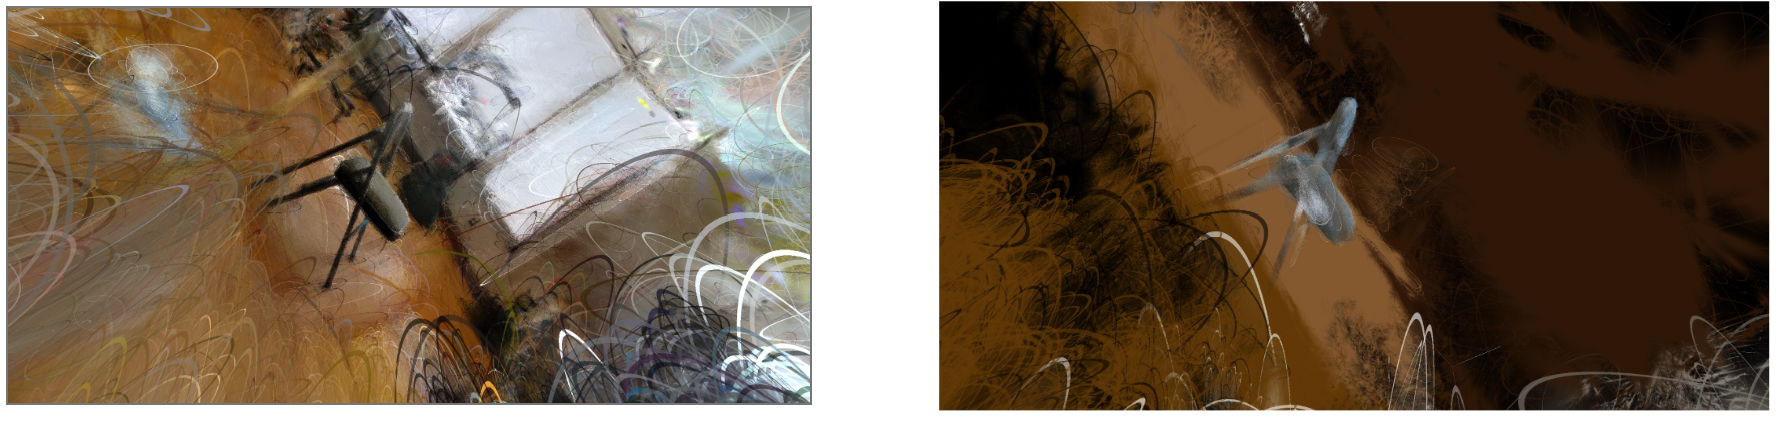
\includegraphics[width=0.92\textwidth]{images/methodology/render_class+render_depth_viewer.png}
    \caption[SuperSplat: RGB vs.\ depth loss]{\textbf{SuperSplat} \cite{supersplat2024} comparison with ellipsoid wireframes.
    \textbf{Left (\code{loss=rgb}):} dense stacks of semi-transparent ellipsoids aligned with viewing rays (stratification in depth).
    \textbf{Right (\code{loss=depth}):} sparser ellipsoid distribution with weaker local layering and reduced structural detail on the foreground object, consistent with a globally smoother depth field.}
    \label{fig:supersplat_rgb_vs_depth}
\end{figure}

\subsection{Failure Modes and Instabilities}
\label{subsec:depth_failure}

Depth supervision inherits limitations of monocular priors: reflective or transparent surfaces, thin structures, and textureless walls can be misestimated by DA3 and then propagated into the Gaussian cloud. Because DA3 depths are computed per view without explicit multi-view fusion, inconsistent pseudo-labels across cameras can create rippling artifacts in $d^{\mathrm{exp}}$. Overly strong depth fitting may also flatten legitimate depth discontinuities (object boundaries), while under-fitting leaves floaters that no longer penalize RGB error.

Practically, $\mathcal{L}_{\mathrm{depth}}$ should be interpreted as a \emph{global geometry regularizer} rather than a replacement for photometric detail. Combining both signals (e.g.\ weighted RGB+$L_1$ depth, or object-masked losses in Section~\ref{sec:bezier_structural}) is left as future work; the present thesis evaluates the two extremes, pure RGB and pure depth, to expose their complementary biases.

\section{Structural Modification via B\'ezier Surfaces}
\label{sec:bezier_structural}

The third methodological axis replaces free 3D Gaussian placement on the full COLMAP cloud with \textbf{object-centric B\'ezier surface patches} \cite{liu2025bezier}. Each patch is a tensor-product B\'ezier surface fitted to a subset of sparse object seed points from the COLMAP point cloud; Gaussians are then sampled on a regular $(u,v)$ grid and optimized jointly with the patch control points. This section covers (i)~how object points are isolated semantically, (ii)~how sparse outliers are removed before fitting, and (iii)~how patches are initialized and coupled to splatting (following subsections).

The pipeline is enabled by \code{bezier\_init\_enabled=True} together with \code{sam2\_semantic\_init\_enabled=True} and a text prompt (e.g.\ \code{sam2\_text\_prompts=["chair"]}). At training startup, \code{VanillaPipeline} runs Grounding DINO + SAM~2, labels COLMAP seed points, and passes \code{metadata["seed\_semantic\_labels"]} to \code{SplatfactoModel} (Section~\ref{sec:huggingface}, Chapter~\ref{chap:tools}).

\subsection{Semantic Object Isolation}
\label{subsec:semantic_isolation}

Object-centric geometry requires associating each COLMAP 3D point $\mathbf{p}_i\in\mathcal{P}$ with a discrete label $\ell_i\in\{0,1,\ldots\}$, where $\ell_i=0$ denotes background and $\ell_i>0$ an object instance or prompt-specific class. This thesis uses the \textbf{Grounded SAM~2} path implemented in \filepath{nerfstudio/models/sam2\_semantics.py}:

\begin{enumerate}
    \item For each training image $I$, \textbf{Grounding DINO} predicts bounding boxes from a text prompt (Section~2.5.1).
    \item \textbf{SAM~2} (\code{SAM2ImagePredictor}) segments each box into a binary mask; masks from multiple prompts are merged into a per-pixel \emph{label map} with prompt-priority rules (later prompts do not overwrite pixels already labeled).
    \item COLMAP 2D tracks (\code{points3D\_image\_ids}, \code{points3D\_points2D\_xy}) project each 3D point into the images where it was observed; the label at the projected pixel votes for that point.
    \item Votes accumulated across all segmented views yield a final label per 3D point (majority / first-hit aggregation in \code{\_labels\_from\_labelmap\_votes}).
\end{enumerate}

Only points with $\ell_i>0$ are retained for B\'ezier fitting; background seeds are discarded before patch generation. Masks can also be exported to the dataparser (\code{convert\_sam2\_labelmaps\_to\_binary\_masks}) for optional foreground--background losses during training (Section~\ref{subsec:mask_losses}).

\begin{figure}[H]
    \centering
    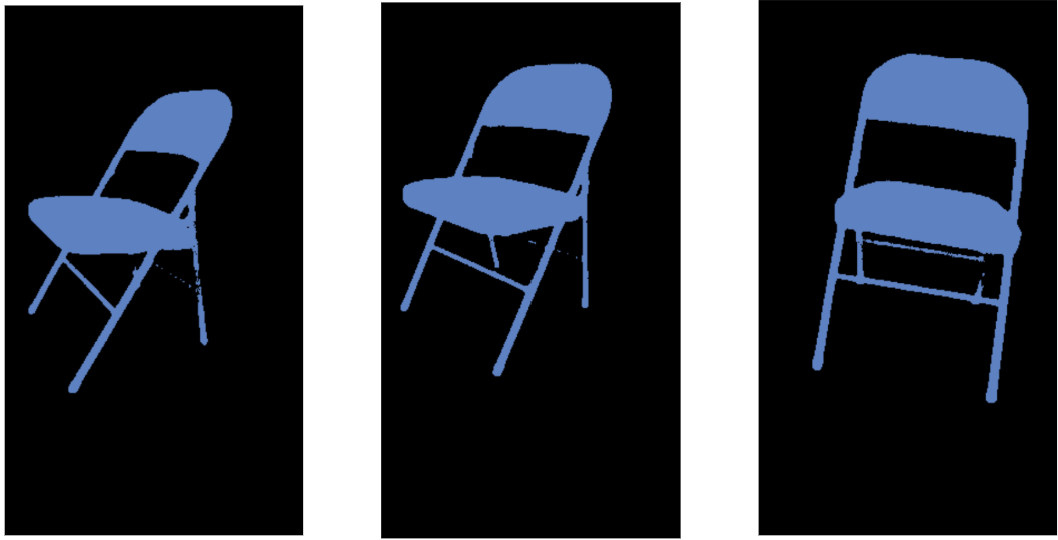
\includegraphics[width=0.92\textwidth]{images/methodology/exaple_segmetation.png}
    \caption{Example SAM~2 masks obtained from a text prompt (here, a chair) on three training views. Each mask defines the image regions that vote for object labels on projected COLMAP seed points.}
    \label{fig:bezier_segmentation_example}
\end{figure}

\paragraph{Configuration.}
Key flags include:
\begin{itemize}
    \item \code{sam2\_text\_prompts};
    \item \code{sam2\_segment\_all\_train\_images} (or an explicit \code{sam2\_segment\_image\_indices} list);
    \item \code{sam2\_segmentation\_output\_dir} (default \filepath{data/grounded\_sam2/}) for label maps and debug visualizations.
\end{itemize}
The dataparser must export full 2D tracks (\code{max\_2D\_matches\_per\_3D\_point} $>0$ or $-1$ for unlimited).

\subsection{Seed Point Preprocessing}
\label{subsec:seed_preprocessing}

Even after semantic filtering, COLMAP triangulation can leave \emph{isolated} seed points far from the object surface; for example, due to matching errors, reflective surfaces, or points on background geometry that received a spurious object label in a single view. Fitting B\'ezier patches to such outliers distorts control nets and produces Gaussians detached from the true shape (Figure~\ref{fig:bezier_outlier_seed}; Figure~\ref{fig:bezier_outliers_output}).

\subsubsection{k-NN Outlier Filtering}
\label{subsec:knn_outlier}

Before patch generation, \texttt{filter\_seed\_points\_outlier\_knn\_mean} in \filepath{splatfacto.py} removes sparse points \emph{per semantic class}. For each label $c$, let $\mathcal{P}_c=\{\mathbf{p}_i:\ell_i=c\}$. For every point $\mathbf{p}_i\in\mathcal{P}_c$, compute the mean distance to its $k$ nearest neighbors within the same class:
\begin{equation}
d_i = \frac{1}{k}\sum_{j=1}^{k}\|\mathbf{p}_i-\mathbf{p}_{i,j}^{(k)}\|,
\qquad
\bar{d}_c = \frac{1}{|\mathcal{P}_c|}\sum_{\mathbf{p}_i\in\mathcal{P}_c} d_i.
\label{eq:knn_mean_dist}
\end{equation}
Point $\mathbf{p}_i$ is kept if $d_i \le \lambda\,\bar{d}_c$ and discarded otherwise, where $\lambda$ and $k$ are set by \code{bezier\_seed\_outlier\_knn\_lambda} and \code{bezier\_seed\_outlier\_knn\_k} (default $k=8$). Setting $\lambda\le 0$ disables filtering. Typical values $\lambda\in[2,3]$ remove only points whose local spacing is far larger than the class average (isolated ``floaters'' in seed space). If all points of a class would be removed, the implementation keeps the full class and logs a warning.

\begin{algorithm}[htbp]
\caption{k-NN outlier filtering of B\'ezier seed points (\code{filter\_seed\_points\_outlier\_knn\_mean})}
\label{alg:knn_outlier}
\begin{algorithmic}[1]
\Require Seed positions $\{\mathbf{p}_i\}$, labels $\{\ell_i\}$, neighbors $k$, multiplier $\lambda$
\Ensure Filtered seeds $(\mathbf{p},\ell)$ with outliers removed per class
\If{$\lambda \le 0$}
    \State \Return all seeds unchanged
\EndIf
\For{each semantic label $c$}
    \State $\mathcal{P}_c \gets \{\mathbf{p}_i : \ell_i = c\}$
    \If{$|\mathcal{P}_c| \le k$}
        \State keep all points in $\mathcal{P}_c$ \Comment{too few points for stable $k$-NN}
    \Else
        \For{each $\mathbf{p}_i \in \mathcal{P}_c$}
            \State $d_i \gets$ mean $\ell_2$ distance to $k$ nearest neighbors in $\mathcal{P}_c$
        \EndFor
        \State $\bar{d}_c \gets \mathrm{mean}_i(d_i)$
        \State keep $\mathbf{p}_i$ iff $d_i \le \lambda\,\bar{d}_c$
    \EndIf
\EndFor
\State \Return concatenation of kept points over all classes
\end{algorithmic}
\end{algorithm}

\begin{lstlisting}[caption={Core loop in \texttt{filter\_seed\_points\_outlier\_knn\_mean} (abridged).},label={lst:knn_outlier}]
dists, _ = k_nearest_sklearn(pts, k)       # (N_c, k) per class
dk = dists.mean(dim=-1)                    # d_i in Eq.~\eqref{eq:knn_mean_dist}
thresh = lambda_mult * dk.mean().clamp_min(1e-8)
keep = dk <= thresh
\end{lstlisting}

The filter is invoked inside \code{SplatfactoModel.populate\_modules} immediately after restricting to object labels ($\ell>0$) and before \code{generate\_bezier\_patches\_from\_labeled\_points} or cube initialization:
\begin{lstlisting}[caption={Call site before B\'ezier patch fitting (\filepath{splatfacto.py}).},label={lst:knn_call}]
seed_xyz_obj, seed_labels_obj, seed_rgb_obj = filter_seed_points_outlier_knn_mean(
    seed_xyz_obj, seed_labels_obj, seed_rgb_obj,
    k=int(self.config.bezier_seed_outlier_knn_k),
    lambda_mult=float(self.config.bezier_seed_outlier_knn_lambda),
)
\end{lstlisting}

\begin{figure}[H]
    \centering
    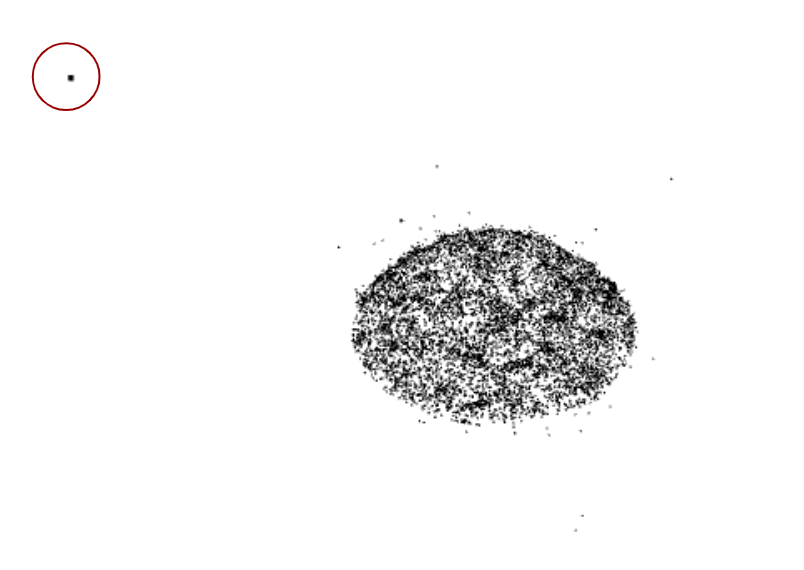
\includegraphics[width=0.55\textwidth]{images/methodology/esempio_outliers.png}
    \caption{Seed outlier \emph{before} $k$-NN filtering: a single mislabeled COLMAP seed (red circle) far from the chair cluster.}
    \label{fig:bezier_outlier_seed}
\end{figure}

\begin{figure}[H]
    \centering
    \begin{subfigure}[b]{0.48\textwidth}
        \centering
        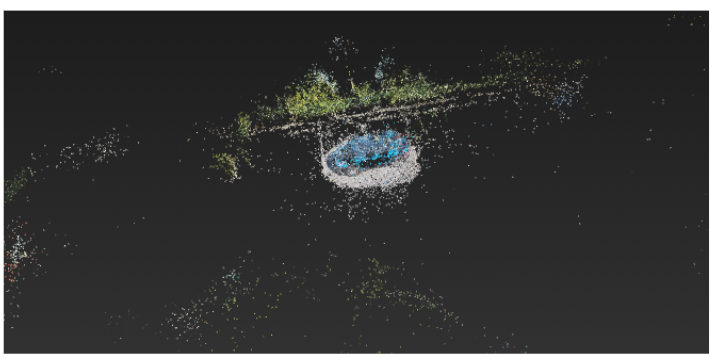
\includegraphics[width=\textwidth]{images/methodology/cloud_point_out.png}
        \caption{Full seed point cloud}
        \label{fig:bezier_outlier_cloud}
    \end{subfigure}
    \hfill
    \begin{subfigure}[b]{0.48\textwidth}
        \centering
        
\includegraphics[width=\textwidth]{{images/methodology/esempio_inizializzazione con outliers.png}}
        \caption{Fitted B\'ezier patches}
        \label{fig:bezier_outlier_gaussians}
    \end{subfigure}
    \caption{B\'ezier initialization when outlier seeds are not removed. \textbf{(a)} COLMAP seed point cloud with all points assigned to the object class (including outliers). \textbf{(b)} 3D visualization of the fitted B\'ezier surfaces warped by those outliers (Open3D).}
    \label{fig:bezier_outliers_output}
\end{figure}

\subsection{B\'ezier Surface Initialization}
\label{subsec:bezier_init}

After semantic filtering and $k$-NN outlier rejection, each object class is represented by one or more tensor-product B\'ezier patches of degree $3\times 3$ (a $4\times 4$ control grid, 16 control points per patch), consistent with Section~2.5.2. This thesis evaluates two \emph{initialization geometries} only:
\begin{itemize}
    \item \textbf{Open-surface mode} (\code{bezier\_init\_enabled=True}, \code{bezier\_cube\_init=False}): patches fitted locally to seed neighborhoods (default \code{bezier\_surface\_mode="open"}).
    \item \textbf{Cube mode} (\code{bezier\_cube\_init=True}): six faces of an axis-aligned bounding box (AABB), each tiled with $k\times k$ patches that share control points on face boundaries and cube edges.
\end{itemize}

\subsubsection{Control Point Estimation}
\label{subsec:bezier_cp_estimation}

\paragraph{Open-surface patches.}
For each semantic label $c$, let $\mathcal{P}_c$ be the filtered seed set. The generator \texttt{generate\_bezier\_patches\_from\_labeled\_points} (\filepath{bezier\_surface.py}) builds \texttt{bezier\_num\_patches\_per\_class} patches as follows:
\begin{enumerate}
    \item \textbf{Patch centers:} select $P$ anchor points in $\mathcal{P}_c$ using farthest-point sampling (FPS, default \texttt{bezier\_center\_sampling="fps"}) or uniform random indices.
    \item \textbf{Local neighborhood:} for each center $\mathbf{c}$, retrieve $K=\texttt{bezier\_knn\_k}$ nearest neighbors in $\mathcal{P}_c$ (typically $K=64$).
    \item \textbf{Planar control grid:} fit a $4\times 4$ control net on the best-fit plane of the neighborhood via PCA (function \texttt{\_create\_planar\_control\_points}): compute the mean $\boldsymbol{\mu}$, take the two principal axes of largest variance, and place control points on a regular grid spanning the projected extent of neighbors in that $(u,v)$ plane. The result is a \emph{planar} initial surface, not a least-squares fit to scattered 3D points.
\end{enumerate}

\begin{algorithm}[htbp]
\caption{Open-mode B\'ezier control-point initialization (per class, per patch)}
\label{alg:bezier_cp_open}
\begin{algorithmic}[1]
\Require Filtered seeds $\mathcal{P}_c$, number of patches $P$, neighbors $K$, grid size $G{=}4$
\State $\mathcal{C} \gets \mathrm{FPS}(\mathcal{P}_c, P)$ \Comment{or random centers}
\For{each center $\mathbf{c} \in \mathcal{C}$}
    \State $\mathcal{N} \gets k\mathrm{NN}(\mathcal{P}_c, \mathbf{c}, K)$
    \State $(\mathbf{u},\mathbf{v}) \gets$ first two principal axes of $\mathcal{N}$ (PCA)
    \State Project $\mathcal{N}$ onto $(\mathbf{u},\mathbf{v})$; build $G\times G$ grid in that plane
    \State Store control net $\mathbf{p}_{i,j}\in\mathbb{R}^3$, $i,j\in\{0,\ldots,G{-}1\}$
\EndFor
\end{algorithmic}
\end{algorithm}

\begin{lstlisting}[caption={Planar control grid from a $k$-NN neighborhood (\filepath{bezier\_surface.py}).},label={lst:planar_cp}]
mu = neighbors.mean(dim=0)
X = neighbors - mu
C = (X.T @ X) / (K - 1)
evecs = torch.linalg.eigh(C).eigenvectors
u_axis, v_axis = evecs[:, -1], evecs[:, -2]
# GxG grid along projected min/max extents -> (G, G, 3) control points
\end{lstlisting}

\paragraph{Cube-mode patches.}
When \code{bezier\_cube\_init=True}, control points are \emph{not} fitted from local neighborhoods. Instead, \code{generate\_bezier\_cube\_from\_labeled\_points} computes the AABB $[\mathbf{b}_{\min},\mathbf{b}_{\max}]$ of $\mathcal{P}_c$, inflates degenerate axes by a tiny margin, and calls \code{build\_cube\_bezier\_control\_points}:
\begin{itemize}
    \item Each of the six box faces carries a regular $n_{\mathrm{cp}}\times n_{\mathrm{cp}}$ lattice of world-space control points, with $n_{\mathrm{cp}} = 3k+1$ for cubic patches ($k=\texttt{bezier\_cube\_k}$ patches per face edge).
    \item Face lattices are concatenated; coincident points at edges and corners are merged via \code{torch.unique}, yielding a single tensor \code{bezier\_cube\_shared\_cp} of unique positions.
    \item An \code{index\_map} of shape $(6k^2,4,4)$ maps each face patch to indices into the shared tensor. Adjacent patches therefore share boundary control points by construction ($C^0$ continuity along cube edges), without a separate ``shell'' or closed-volume model (see Figure~\ref{fig:bezier_cube_box}).
\end{itemize}

\subsubsection{Surface Sampling and Gaussian Seeding}
\label{subsec:bezier_surface_sampling}

Control points define a patch $\mathbf{S}(u,v)$ via Bernstein blending (Section~2.5.2, Figure~\ref{fig:bezier_surface_example}). At initialization, each patch is uniformly sampled on
\begin{align}
u_i &= \frac{i}{N_u-1},\quad v_j = \frac{j}{N_v-1}, \\
i &\in \{0,\ldots,N_u-1\},\quad j \in \{0,\ldots,N_v-1\},
\end{align}
with $N_u=\texttt{bezier\_num\_u}$ and $N_v=\texttt{bezier\_num\_v}$ (defaults $20\times 20$). Sample positions $\mathbf{x}_{i,j}=\mathbf{S}(u_i,v_j)$ become Gaussian \textbf{means}.

\paragraph{Local tangent frame.}
For each sample, central finite differences on the grid approximate partial tangents $\partial_u\mathbf{S}$ and $\partial_v\mathbf{S}$; border samples use forward/backward stencils. Unit tangents $\mathbf{t}_u,\mathbf{t}_v$ and normal $\mathbf{n}=\mathbf{t}_u\times\mathbf{t}_v$ (re-orthogonalized) form a rotation matrix $\mathbf{R}=[\mathbf{t}_u\;\mathbf{t}_v\;\mathbf{n}]$, converted to quaternions for \texttt{gsplat}. This aligns each Gaussian's anisotropy with the local surface geometry.

\paragraph{Anisotropic scales.}
In the local frame $\mathbf{R}=[\mathbf{t}_u\;\mathbf{t}_v\;\mathbf{n}]$, each ellipsoid has semi-axis lengths $(\sigma_u,\sigma_v,\sigma_n)$ along the tangent directions and the surface normal. Adjacent sample spacing on the patch sets the \emph{tangential} extents; $\rho$ and $\alpha$ map grid spacing to world-space axis lengths:
\[
\sigma_u = \frac{\|\mathbf{x}_{i+1,j}-\mathbf{x}_{i,j}\|}{\rho},\qquad
\sigma_v = \frac{\|\mathbf{x}_{i,j+1}-\mathbf{x}_{i,j}\|}{\rho},
\qquad
\sigma_n = \frac{\alpha}{\rho},
\]
with $\rho=\texttt{bezier\_rho}$ (default $20$) and $\alpha=\texttt{bezier\_alpha}$ (default $1$). Thus $\rho$ shrinks or enlarges the in-plane footprint relative to the distance between lattice samples (larger $\rho$ $\Rightarrow$ narrower splats along $\mathbf{t}_u,\mathbf{t}_v$ and more overlap between neighbors on the surface), whereas $\alpha$ sets the initial \emph{normal} thickness $\sigma_n$ independently of local spacing (larger $\alpha$ $\Rightarrow$ thicker support off the surface). Log-scales passed to \texttt{gsplat} are $\log(\sigma_u,\sigma_v,\sigma_n)$.

\paragraph{Appearance and semantics.}
Per-patch color is the mean RGB of seed points in that semantic class; all $N_u N_v$ Gaussians on the patch inherit it as flat SH DC coefficients (\texttt{RGB2SH}), with higher bands zero unless \texttt{patch\_textures} override color each forward (Section~\ref{subsec:bezier_textures}). Semantic labels are stored in \code{gaussian\_semantic\_labels}. In \textbf{open mode}, the $4\times 4$ control nets are registered as \code{bezier\_open\_cp} and re-sampled every forward pass so rendering gradients update geometry. In \textbf{cube mode}, \code{bezier\_cube\_shared\_cp} plays the same role with patches indexed through \code{bezier\_cube\_index\_map}.

\begin{algorithm}[htbp]
\caption{From B\'ezier patch samples to initial Gaussian parameters (open mode)}
\label{alg:bezier_gaussian_seed}
\begin{algorithmic}[1]
\Require Control net $\{\mathbf{p}_{i,j}\}$, grid sizes $N_u,N_v$, $\rho$, $\alpha$
\State $\mathbf{X} \gets$ \texttt{BezierSurfacePatch.sample}($N_u,N_v$) \Comment{$(N_u,N_v,3)$}
\State $\mathbf{t}_u,\mathbf{t}_v \gets$ finite differences on $\mathbf{X}$; $\mathbf{n} \gets \mathbf{t}_u \times \mathbf{t}_v$
\State $\mathbf{q} \gets \mathrm{rotmat2quat}([\mathbf{t}_u,\mathbf{t}_v,\mathbf{n}])$
\State $\sigma_u,\sigma_v \gets$ neighbor sample distances $/\rho$; $\sigma_n \gets \alpha/\rho$
\State Register means $=\mathrm{vec}(\mathbf{X})$, scales $=\log(\sigma_u,\sigma_v,\sigma_n)$, quats $=\mathbf{q}$
\end{algorithmic}
\end{algorithm}

\begin{lstlisting}[caption={Open-mode sampling and Gaussian frames (\filepath{splatfacto.py}, simplified).},label={lst:bezier_sample}]
X = patch.sample(num_u=Nu, num_v=Nv)          # (Nu, Nv, 3)
# finite differences -> tu, tv, n -> quaternions
sigma_u = ||X[i+1,j]-X[i,j]|| / rho
scales_log = log([sigma_u, sigma_v, alpha/rho])
means = X.reshape(-1, 3)
\end{lstlisting}

\subsection{B\'ezier Representations}
\label{subsec:bezier_representations}

The two representations differ in \emph{how} control points are laid out (local PCA planes vs.\ a shared AABB lattice), not in the rendering or loss machinery. Both are evaluated on the same scenes in Chapter~\ref{chap:results}; the choice is treated as an initialization prior rather than a hard partition of object categories.

\subsubsection{Open-Surface Mode}
\label{subsec:bezier_open}

Open mode places $P$ independent $4\times 4$ patches on the object: each FPS center picks a neighborhood of seeds and initializes control points on a local PCA plane (\code{bezier\_open\_cp[s,i,j,:]}, Section~\ref{subsec:bezier_cp_estimation}). Patch orientations can differ from one another, which can help when seeds form several oriented sheets or highly non-convex visible regions; it is not a requirement for such objects, and cube mode is compared on the same data. During training, \code{\_bezier\_open\_resample\_means\_scales} recomputes all Gaussian means and covariances from the \emph{current} control nets at every iteration, so photometric (or mask) losses back-propagate into $\mathbf{p}_{i,j}$ without relying on adaptive densification on the object (densification is skipped when open/cube reparameterization is active).

Optional per-patch \code{patch\_textures} grids ($T\times T\times 4$, default $T=8$) supply RGBA at each $(u,v)$ sample, overriding spherical-harmonic color and opacity on the surface. Optional \code{bezier\_open\_cp\_l2\_lambda} penalizes control-point drift from initialization.

Configuration summary: \code{bezier\_num\_patches\_per\_class}, \code{bezier\_knn\_k}, \code{bezier\_center\_sampling}, \code{bezier\_num\_u/v}, \code{bezier\_rho}, \code{bezier\_alpha}.

\subsubsection{Cube-Based B\'ezier Surfaces}
\label{subsec:bezier_cube}

Cube mode anchors control points to the six faces of the object AABB $[\mathbf{b}_{\min},\mathbf{b}_{\max}]$: a regular lattice per face, with vertices merged at edges and corners into \code{bezier\_cube\_shared\_cp}. The scaffold is box-shaped at initialization, but training still deforms the lattice; in the reported experiments it performed well on both test scenes (pizza and parking meter), not only on strictly box-like geometry. The main structural difference from open mode is global layout and enforced $C^0$ sharing between face patches rather than independent PCA planes.

Given AABB $[\mathbf{b}_{\min},\mathbf{b}_{\max}]$ and $k=\texttt{bezier\_cube\_k}$:
\begin{itemize}
    \item Total patches $S = 6k^2$ (e.g.\ $k{=}1 \Rightarrow 6$ patches, one per face).
    \item All patches read control positions from one shared vector \code{bezier\_cube\_shared\_cp} of length $N_{\mathrm{unique}}$; \code{bezier\_cube\_index\_map[s]} selects the $4\times 4$ indices for patch $s$.
    \item Training uses the same open-mode resampling path (\code{bezier\_surface\_mode} must remain \code{"open"}); only the initialization of control points differs.
\end{itemize}

\begin{lstlisting}[caption={Cube AABB and shared control points (\filepath{bezier\_surface.py}).},label={lst:bezier_cube}]
bbox_min, bbox_max = pts.min(0), pts.max(0)
unique_cp, index_map = build_cube_bezier_control_points(
    bbox_min, bbox_max, k=bezier_cube_k, grid_size=4)
# index_map: (6*k*k, 4, 4) -> indices into unique_cp
\end{lstlisting}

\begin{figure}[H]
    \centering
    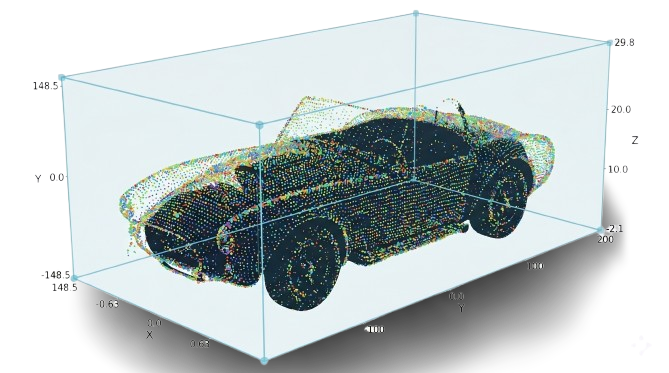
\includegraphics[width=0.72\textwidth]{images/methodology/box_bezier.png}
    \caption{Cube-mode initialization for a segmented object (classic car): COLMAP seed points (colored by SfM RGB) lie inside the object AABB $[\mathbf{b}_{\min},\mathbf{b}_{\max}]$ (semi-transparent box). The six faces of this box host the shared B\'ezier control lattice; $k\times k$ cubic patches per face are anchored to the lattice vertices merged at edges and corners.}
    \label{fig:bezier_cube_box}
\end{figure}

Neither mode implements a closed volumetric shell (no inner surface $S_{\mathrm{in}}$ or thickness layers). Empirically, cube mode with outlier filtering and FgBg losses gave the most regular exported meshes on both objects (Section~\ref{subsec:results_best_quant}), while open mode with FPS and outliers remained competitive on some Chamfer curves (e.g.\ pizza, Figure~\ref{fig:pizza_best_chamfer_bid}). Open initialization may be worth trying when seeds are fragmented or strongly curved locally; cube initialization is a strong default when a coherent six-face lattice is acceptable.

\subsection{B\'ezier Surface Parameterization}
\label{subsec:bezier_textures}

Beyond geometry, each surface patch $s$ can carry a learnable \textbf{texture grid}
\[
\mathbf{T}_s \in \mathbb{R}^{T\times T\times 4},
\qquad T=\texttt{bezier\_texture\_size}\ \ (\text{default }8),
\]
stored as \texttt{patch\_textures} and initialized uniformly in $[0,0.5]$ before sigmoid. For every Gaussian tied to patch $s$ at indices $(u_i,v_j)$ on the $N_u\times N_v$ sampling grid, texture coordinates are obtained by nearest indexing:
\begin{equation}
t_u = \mathrm{round}\!\left(u_i\,\frac{T-1}{N_u-1}\right),\qquad
t_v = \mathrm{round}\!\left(v_j\,\frac{T-1}{N_v-1}\right),
\label{eq:texture_index}
\end{equation}
and the pre-activation vector $\boldsymbol{\tau}=\mathbf{T}_s[t_u,t_v]\in\mathbb{R}^4$ is mapped through $\sigma(\cdot)$ (sigmoid) to RGBA in $[0,1]^4$. During \texttt{get\_outputs}, these values \emph{override} the static spherical-harmonic color and the stored opacity logit for that Gaussian for the current forward pass (Listing~\ref{lst:texture_override}).

\paragraph{In other words.}
Per patch, one defines a $T\times T$ grid of learnable color tiles (RGBA) and an $N_u\times N_v$ grid of Gaussians on the same surface. Each Gaussian keeps fixed indices $(s,i,j)$ (patch id and cell on the sampling lattice). At render time, $(i,j)$ is mapped to a tile $(t_u,t_v)$ via Eq.~\eqref{eq:texture_index}; that tile sets the splat's color and opacity for the forward pass. Under \textbf{code defaults} ($T{=}8$, $N_u{=}N_v{=}20$), $T^2{=}64$ tiles serve $N_u N_v{=}400$ Gaussians, so many splats share one tile. In \textbf{all B\'ezier runs reported in Chapter~\ref{chap:results}}, we instead set $T=N_u=N_v$ (typically $30$), giving a one-to-one assignment $t_u{=}i$, $t_v{=}j$ and one learnable RGBA tile per Gaussian on each patch; other hyperparameters (patch count, $\rho$, cube vs.\ open) vary by ablation, but this coupling was kept fixed so appearance resolution matches the sampling lattice.

\begin{lstlisting}[caption={Texture lookup in \texttt{get\_outputs} (open/cube mode).},label={lst:texture_override}]
tu = (uu * (T_tex - 1) / max(1, Nu - 1)).long()
tv = (vv * (T_tex - 1) / max(1, Nv - 1)).long()
rgba_01 = torch.sigmoid(patch_textures[pp, tu, tv])  # (N, 4)
features_dc = RGB2SH(rgba_01[:, :3])
opacities = torch.logit(rgba_01[:, 3:4].clamp(1e-6, 1-1e-6))
\end{lstlisting}

Higher-order SH bands are zeroed so view-dependent effects on the object surface are carried by the texture grid (and by joint motion of control points), not by per-Gaussian SH rest coefficients.

\subsection{Gaussian Parameter Initialization from B\'ezier Surfaces}
\label{subsec:gaussian_init}

Each sample $(s,i,j)$ on the uniform $(u,v)$ grid defines one 3D Gaussian primitive. Following Section~2.3.4, its learnable state is
\[
\boldsymbol{\Theta}_{s,i,j}=
\bigl\{
\boldsymbol{\mu}_{s,i,j},\,
\mathbf{s}_{s,i,j},\,
\mathbf{q}_{s,i,j},\,
o_{s,i,j},\,
\mathbf{f}_{s,i,j}
\bigr\},
\]
where $\boldsymbol{\mu}$ is the mean, $\mathbf{s}\in\mathbb{R}^3$ the \emph{log-scale} vector stored in the optimizer, $\mathbf{q}\in\mathbb{R}^4$ the unit quaternion (xyzw convention for \texttt{gsplat}), $o$ the opacity after sigmoid, and $\mathbf{f}$ the appearance coefficients (spherical harmonics or logits). Initialization is deterministic given control points $\{\mathbf{p}_{a,b}\}$ and configuration $(N_u,N_v,\rho,\alpha)$; index buffers \texttt{bezier\_open\_patch\_idx}, \texttt{bezier\_open\_u\_idx}, \texttt{bezier\_open\_v\_idx} record which $(s,i,j)$ each Gaussian represents for the lifetime of training.

\subsubsection{Mean positions}
\label{subsubsec:init_means}

Let $\mathbf{S}_s(u,v)$ be the $4\times 4$ B\'ezier patch for surface $s$. Discrete parameters $u_i=i/(N_u-1)$, $v_j=j/(N_v-1)$ yield sample positions
\begin{equation}
\boldsymbol{\mu}_{s,i,j}=\mathbf{S}_s(u_i,v_j)
=\sum_{a=0}^{3}\sum_{b=0}^{3} B_a^{3}(u_i)\,B_b^{3}(v_j)\,\mathbf{p}_{s,a,b},
\label{eq:gaussian_mean_bezier}
\end{equation}
with Bernstein polynomials $B_k^{3}$ as in Section~2.5.2. Stacking all patches gives $N_{\mathrm{g}}=S\cdot N_u\cdot N_v$ means. In \textbf{open/cube training}, $\boldsymbol{\mu}$ is \emph{recomputed} from the current control nets every forward pass via \texttt{\_bezier\_open\_resample\_means\_scales}, so gradients on rendering losses update $\mathbf{p}_{a,b}$ even though a \texttt{means} parameter tensor exists from init.

\subsubsection{Local tangent frame and quaternion}
\label{subsubsec:init_quat}

Let $\mathbf{X}_s\in\mathbb{R}^{N_u\times N_v\times 3}$ be the sampled grid for patch $s$. Discrete tangents use central differences in the interior and one-sided stencils on borders:
\begin{align}
\partial_u \mathbf{X}_{s,i,j} &\approx
\begin{cases}
\mathbf{X}_{s,i+1,j}-\mathbf{X}_{s,i-1,j} & 1\le i\le N_u-2,\\
\mathbf{X}_{s,1,j}-\mathbf{X}_{s,0,j} & i=0,\\
\mathbf{X}_{s,N_u-1,j}-\mathbf{X}_{s,N_u-2,j} & i=N_u-1,
\end{cases}
\label{eq:fd_u}\\
\partial_v \mathbf{X}_{s,i,j} &\approx
\text{(analogous along $j$)}.
\label{eq:fd_v}
\end{align}
Unit vectors $\mathbf{t}_u=\partial_u\mathbf{X}/\|\partial_u\mathbf{X}\|$, $\mathbf{t}_v=\partial_v\mathbf{X}/\|\partial_v\mathbf{X}\|$, and normal $\mathbf{n}=(\mathbf{t}_u\times\mathbf{t}_v)/\|\mathbf{t}_u\times\mathbf{t}_v\|$ are re-orthogonalized ($\mathbf{t}_v\leftarrow \mathbf{n}\times\mathbf{t}_u$) to form a right-handed frame. The rotation matrix $\mathbf{R}_{s,i,j}=[\mathbf{t}_u\;\mathbf{t}_v\;\mathbf{n}]\in SO(3)$ is converted to a quaternion $\mathbf{q}_{s,i,j}$ using COLMAP's \code{rotmat2qvec} and a wxyz$\rightarrow$xyzw reordering to match \code{gsplat}.

In the implementation, $\mathbf{q}_{s,i,j}$ is stored once at initialization in \code{gauss\_params["quats"]}; it is \textbf{not} refreshed when control points move during training (only $\boldsymbol{\mu}$ and $\mathbf{s}$ are resampled from the deformed surface). The initial frame therefore encodes the surface orientation at step zero.

\subsubsection{Anisotropic scales (log-space)}
\label{subsubsec:init_scales}

Gaussian covariance is modeled as $\boldsymbol{\Sigma}=\mathbf{R}\,\mathrm{diag}(\sigma_u^2,\sigma_v^2,\sigma_n^2)\,\mathbf{R}^\top$ (Section~2.3.4). Axis lengths are tied to the sampling grid and hyperparameters $\rho>0$, $\alpha>0$:
\begin{align}
\sigma_{u,s,i,j} &= \frac{\bigl\|\mathbf{X}_{s,i+1,j}-\mathbf{X}_{s,i,j}\bigr\|}{\rho}, \\
\sigma_{v,s,i,j} &= \frac{\bigl\|\mathbf{X}_{s,i,j+1}-\mathbf{X}_{s,i,j}\bigr\|}{\rho}, \\
\sigma_{n,s,i,j} &= \frac{\alpha}{\rho},
\label{eq:gaussian_scales}
\end{align}
with $\sigma_{u}$ at $i=N_u-1$ (and $\sigma_v$ at $j=N_v-1$) copied from the previous sample. The optimizer stores
\begin{equation}
\mathbf{s}_{s,i,j}=\log\bigl(\max(\boldsymbol{\sigma}_{s,i,j},\varepsilon)\bigr)\in\mathbb{R}^3,
\qquad
\boldsymbol{\sigma}_{s,i,j}=(\sigma_u,\sigma_v,\sigma_n)^\top,
\label{eq:log_scales}
\end{equation}
and \texttt{gsplat} uses $\mathrm{diag}(\exp(\mathbf{s}))$ inside the ellipsoid (same log-scale convention as in Section~2.3.4, not an extra modeling choice).

\paragraph{Role of $\rho$ and $\alpha$.}
Both hyperparameters act on the \textbf{geometric extent} of each Gaussian in the patch frame, not on its color or opacity. Let $\Delta_u=\|\mathbf{X}_{s,i+1,j}-\mathbf{X}_{s,i,j}\|$ be the Euclidean spacing between consecutive $(u,v)$ samples after surface deformation (and $\Delta_v$ analogously along $v$).
\begin{itemize}
    \item $\rho$ (\texttt{bezier\_rho}) compares tangential semi-axes to that spacing: $\sigma_u\approx \Delta_u/\rho$ and $\sigma_v\approx \Delta_v/\rho$. A splat therefore occupies roughly a $1/\rho$ fraction of the distance to its neighbor along each tangent. \textbf{Larger $\rho$} yields thinner, more numerous overlapping ellipsoids on the lattice (finer tiling of the surface in the $(u,v)$ plane); \textbf{smaller $\rho$} yields wider footprints that can over-blur detail or leave gaps if opacity is low. Because $\sigma_n=\alpha/\rho$, increasing $\rho$ also thins the shell along $\mathbf{n}$ unless $\alpha$ is raised.
    \item $\alpha$ (\texttt{bezier\_alpha}) sets only the normal semi-axis $\sigma_n=\alpha/\rho$, i.e.\ how thick the initial shell is \emph{perpendicular} to the surface. It does not depend on $\Delta_u,\Delta_v$: two samples on a stretched patch keep the same $\sigma_n$ until $\rho$ or $\alpha$ change. \textbf{Larger $\alpha$} makes each Gaussian more volumetric (less pancake-like); \textbf{smaller $\alpha$} keeps splats as thin sheets hugging $\mathbf{S}(u,v)$, which matches the B\'ezier-surface prior but offers less margin to represent offset geometry or slight misalignment between surface and true object.
\end{itemize}
In open/cube mode these formulas are reapplied every forward pass, so $(\rho,\alpha)$ remain the main levers on ellipsoid shape while control points move; quaternions are fixed at initialization (Section~\ref{subsubsec:init_quat}), so $\sigma_u,\sigma_v,\sigma_n$ always refer to the same local axes $\mathbf{t}_u,\mathbf{t}_v,\mathbf{n}$.

During training (open/cube), $\mathbf{s}$ is recomputed from the \emph{current} $\mathbf{X}$ via Eq.~\eqref{eq:gaussian_scales} (Listing~\ref{lst:open_resample_scales}).

\begin{lstlisting}[caption={Log-scale recomputation in \code{\_bezier\_open\_resample\_means\_scales}.},label={lst:open_resample_scales}]
du = X[:, 1:, :, :] - X[:, :-1, :, :]
sigma_u = ||du|| / rho   # pad last row
sigma_n = alpha / rho
scales_log = log(stack([sigma_u, sigma_v, sigma_n], dim=-1))
\end{lstlisting}

\subsubsection{Opacity}
\label{subsubsec:init_opacity}

Opacity is parameterized as $o=\sigma(\eta)$ with learnable logit $\eta$. At B\'ezier initialization all Gaussians share
\begin{equation}
\eta_{s,i,j}=\mathrm{logit}(0.1)=\log\frac{0.1}{0.9},
\label{eq:init_opacity_logit}
\end{equation}
i.e.\ initial visible opacity $o\approx 0.1$. When \texttt{patch\_textures} are enabled, $\eta$ is replaced at each forward by $\mathrm{logit}(\alpha_{s,i,j})$ where $\alpha_{s,i,j}$ is the sigmoid of the texture's fourth channel (Section~\ref{subsec:bezier_textures}).

\subsubsection{Summary of stored tensors}
\label{subsubsec:init_summary}

Table~\ref{tab:gaussian_init_bezier} lists the mapping from mathematical quantities to \code{SplatfactoModel} fields after B\'ezier init.

\begin{table}[htbp]
\centering
\footnotesize
\caption{B\'ezier-mode Gaussian initialization (open/cube). ``Resampled'' = recomputed each forward from current control points.}
\label{tab:gaussian_init_bezier}
\begin{tabularx}{\linewidth}{@{}l l >{\raggedright\arraybackslash}X >{\raggedright\arraybackslash}X@{}}
\toprule
Quantity & Symbol & Tensor / buffer & Updated during training \\
\midrule
Mean & $\boldsymbol{\mu}$ & \code{means} (then resampled) & Resampled from CP \\
Log-scale & $\mathbf{s}$ & \code{scales} (then resampled) & Resampled from CP \\
Quaternion & $\mathbf{q}$ & \code{quats} & Fixed after init \\
Opacity logit & $\eta$ & \code{opacities} & Learned; or from texture \\
SH coefficients & $\mathbf{f}$ & \code{features\_dc}, \code{features\_rest} & Learned; or from texture \\
Patch indices & $(s,i,j)$ & \code{bezier\_open\_*\_idx} & Fixed buffers \\
Control points & $\mathbf{p}_{a,b}$ & \code{bezier\_open\_cp} / \code{bezier\_cube\_shared\_cp} & Optimized \\
Texture & $\mathbf{T}_s$ & \code{patch\_textures} & Optimized \\
\bottomrule
\end{tabularx}
\end{table}

\paragraph{Contrast with classical COLMAP initialization.}
If B\'ezier init is disabled, means are COLMAP points, scales are $\log(\bar{d})$ with $\bar{d}$ the mean distance to three nearest neighbors (isotropic), quaternions are random unit quaternions, and colors come from per-point SfM RGB via \texttt{RGB2SH}. B\'ezier initialization replaces the unstructured cloud with a structured $N_u\times N_v$ lattice on $\mathbf{S}(u,v)$, oriented anisotropic covariances aligned to $\mathbf{t}_u,\mathbf{t}_v,\mathbf{n}$, and fixed semantic indices per Gaussian.

\begin{lstlisting}[caption={Classical COLMAP scale init (fallback path, \filepath{splatfacto.py}).},label={lst:classic_scale}]
distances, _ = k_nearest_sklearn(means, k=3)
avg_dist = distances.mean(dim=-1).clamp(min=1e-6)
scales = torch.nn.Parameter(torch.log(avg_dist.repeat(1, 3)))  # isotropic log-scale
\end{lstlisting}

\subsection{Integration into the Splatting and Training Pipeline}
\label{subsec:bezier_pipeline}

B\'ezier-mode Splatfacto reuses the standard \code{gsplat} rasterizer and Nerfstudio trainer; the difference is \emph{which} tensors are optimized and how geometry is refreshed each step. Training still follows the loop of Chapter~\ref{chap:tools}: sample a full-frame camera, then \code{get\_outputs}, rasterization, \code{get\_loss\_dict}, backward pass, and optimizer step.

\subsubsection{Parameter registration and optimizer groups}
\label{subsubsec:bezier_optimizer}

Gaussian attributes live in \code{gauss\_params}. In open/cube B\'ezier mode, \code{get\_gaussian\_param\_groups} \emph{rebinds} the optimizer:
\begin{itemize}
    \item \textbf{Geometry:} \code{bezier\_open\_cp} $(S,4,4,3)$ or \code{bezier\_cube\_shared\_cp} $(N_{\mathrm{unique}},3)$ is registered under the \code{means} group (replacing free 3D positions). The classical \code{scales} group is \emph{dropped} from the optimizer (Listing~\ref{lst:param_groups}).
    \item \textbf{Appearance:} optional \code{patch\_textures} $(S,T,T,4)$ in group \code{patch\_textures} (lr $2.5\times 10^{-3}$).
    \item \textbf{Remaining splats:} \code{quats}, \code{features\_dc/rest}, \code{opacities} keep their classical groups unless textures override color/opacity in the forward pass (then gradients flow into $\mathbf{T}_s$ instead).
    \item \textbf{Cameras / bilateral:} unchanged (\code{camera\_opt}, \code{bilateral\_grid} if enabled).
\end{itemize}

\paragraph{Why \texttt{scales} are omitted from the optimizer.}
In standard 3DGS, \code{gauss\_params["scales"]} is a learnable tensor: Adam updates it and the rasterizer reads $\exp(\mathbf{s})$ directly. In open/cube B\'ezier mode this is \emph{not} the case: each forward pass recomputes $\boldsymbol{\mu}_{s,i,j}$ and $\mathbf{s}_{s,i,j}=\log\boldsymbol{\sigma}_{s,i,j}$ from the \emph{current} control net via Eq.~\eqref{eq:reparam_chain} and \eqref{eq:gaussian_scales} (\texttt{\_bezier\_open\_resample\_means\_scales}), then passes those tensors to \texttt{gsplat}. Ellipsoid sizes therefore follow automatically from surface sampling density and $(\rho,\alpha)$; they are still used in rendering, but they are not independent degrees of freedom. Keeping \code{scales} in the optimizer would apply updates that the next forward overwrites, while the loss gradients on $\mathbf{s}$ already reach the control points through $\partial\mathbf{s}/\partial\mathbf{p}$. What is learned is the surface geometry (and optionally \texttt{patch\_textures}), not a separate log-scale vector per Gaussian (e.g.\ $N_u N_v$ scalars per patch).

Default learning rates in \texttt{method\_configs.py} mirror 3DGS: control-net tensors use the same exponential decay as means ($1.6\times 10^{-4}\rightarrow 1.6\times 10^{-6}$ over 30k steps). Listing~\ref{lst:param_groups} shows the registration logic.

\begin{lstlisting}[caption={Open/cube B\'ezier parameter groups (\filepath{splatfacto.py}).},label={lst:param_groups}]
if hasattr(self, "bezier_open_cp"):
    gps["means"] = [self.bezier_open_cp]   # CP tensor uses the "means" slot
    gps.pop("scales", None)
    if hasattr(self, "patch_textures"):
        gps["patch_textures"] = [self.patch_textures]
\end{lstlisting}

\paragraph{Adaptive densification disabled.}
Classical Splatfacto clones/splits/prunes Gaussians from view-space gradient statistics. In B\'ezier open/cube mode this is turned off (\code{skip\_densify=True} in \code{get\_outputs}), because the Gaussian count and $(s,i,j)$ indices are fixed by the $(N_u,N_v)$ lattice on each patch. All geometric degrees of freedom are in the control nets (and textures), not in the number of primitives.

\subsection{Gradient propagation to control points}
\label{subsec:bezier_gradients}

Differentiable rasterization \cite{kerbl2023gaussian} back-propagates $\partial\mathcal{L}/\partial\mathbf{C}$ to per-Gaussian color and opacity, then through projection to 3D means, covariances, and opacities. Figure~\ref{fig:3dgs_grad_graph} reproduces the standard 3DGS backward graph (screen-space Gaussian $G'$, projection $P$, covariance $\boldsymbol{\Sigma}=RSS^\top R^\top$, sigmoid opacity).

\begin{figure}[H]
    \centering
    \resizebox{0.98\textwidth}{!}{%
    \begin{tikzpicture}[
        node distance=0.38cm and 0.55cm,
        every node/.style={rectangle, draw, align=center, font=\scriptsize, inner sep=2.5pt},
        leaf/.style={fill=gray!15},
        grad/.style={-{Stealth}, red!70!black, thick},
        fwd/.style={-{Stealth}, thick},
    ]
        \node (L) {$\mathcal{L}$};
        \node[below=of L] (Ci) {$C_i=\sum_n c_n\,\alpha_n\!\prod_{j<n}(1{-}\alpha_j)$};
        \node[below left=0.95cm and 0.05cm of Ci, leaf] (cn) {$c_n$};
        \node[below right=0.95cm and 0.05cm of Ci] (an) {$\alpha_n=o_n\,G'_n$};
        \node[below left=0.85cm and 0.15cm of an, leaf] (on) {$o_n=\sigma(\eta_n)$};
        \node[below right=0.85cm and 0.15cm of an] (Gn) {$G'_n(\mathbf{x})=\exp\!\bigl(-\tfrac12(\mathbf{x}{-}\boldsymbol{\mu}'_n)^\top\!\boldsymbol{\Sigma}_n'^{-1}(\cdot)\bigr)$};
        \node[below left=of Gn] (mup) {$\boldsymbol{\mu}'_n=P\boldsymbol{\mu}_n$};
        \node[below=of mup, leaf] (mu) {$\boldsymbol{\mu}_n$};
        \node[below right=of Gn] (Sp) {$\boldsymbol{\Sigma}'_n=J W\boldsymbol{\Sigma}_n W^\top J^\top$};
        \node[below=of Sp] (Sig) {$\boldsymbol{\Sigma}_n=R S S^\top R^\top$};
        \node[below left=of Sig] (sexp) {$S=\mathrm{diag}(\exp(\mathbf{s}_n))$};
        \node[below=of sexp, leaf] (sn) {$\mathbf{s}_n$};
        \node[below right=of Sig] (qrot) {$R=R(\mathbf{q}_n)$};
        \node[below=of qrot, leaf] (qn) {$\mathbf{q}_n$};
        % forward (parameter $\rightarrow$ render)
        \draw[fwd] (mu) -- (mup);
        \draw[fwd] (sn) -- (sexp);
        \draw[fwd] (sexp) -- (Sig);
        \draw[fwd] (qn) -- (qrot);
        \draw[fwd] (qrot) -- (Sig);
        \draw[fwd] (Sig) -- (Sp);
        \draw[fwd] (mup) -- (Gn);
        \draw[fwd] (Sp) -- (Gn);
        \draw[fwd] (on) -- (an);
        \draw[fwd] (Gn) -- (an);
        \draw[fwd] (cn) -- (Ci);
        \draw[fwd] (an) -- (Ci);
        \draw[fwd] (Ci) -- (L);
        % backward (loss $\rightarrow$ parameters)
        \draw[grad] (L) -- (Ci);
        \draw[grad] (Ci) -- (cn);
        \draw[grad] (Ci) -- (an);
        \draw[grad] (an) -- (on);
        \draw[grad] (an) -- (Gn);
        \draw[grad] (Gn) -- (mup);
        \draw[grad] (Gn) -- (Sp);
        \draw[grad] (mup) -- (mu);
        \draw[grad] (Sp) -- (Sig);
        \draw[grad] (Sig) -- (sexp);
        \draw[grad] (Sig) -- (qrot);
        \draw[grad] (sexp) -- (sn);
        \draw[grad] (qrot) -- (qn);
    \end{tikzpicture}%
    }
    \caption{Backward pass in 3D Gaussian Splatting (adapted from \cite{kerbl2023gaussian}): loss $\mathcal{L}$ $\rightarrow$ pixel color $C_i$ $\rightarrow$ opacities $\alpha_n$ and colors $c_n$ $\rightarrow$ projected 2D Gaussian $G'_n$ $\rightarrow$ 3D mean $\boldsymbol{\mu}_n$, scales $\mathbf{s}_n$, quaternion $\mathbf{q}_n$. Red arrows indicate gradient flow; black arrows the forward evaluation chain.}
    \label{fig:3dgs_grad_graph}
\end{figure}

\paragraph{B\'ezier extension of the chain.}
In open/cube mode the \emph{effective} 3D position and covariance used at render time are functional outputs of the control net, not the stored \code{gauss\_params["means"]} tensor. Each training step executes
\begin{align}
\mathbf{X}_s &= \mathrm{SampleBezier}\bigl(\{\mathbf{p}_{s,a,b}\}\bigr), \\
\boldsymbol{\mu}_{s,i,j} &= \mathbf{X}_s(u_i,v_j), \\
\mathbf{s}_{s,i,j} &= \log\boldsymbol{\sigma}(\mathbf{X}_s,\rho,\alpha),
\label{eq:reparam_chain}
\end{align}
before calling \code{gsplat.rasterization}. Therefore, by the chain rule,
\begin{equation}
\frac{\partial\mathcal{L}}{\partial \mathbf{p}_{s,a,b}}
=
\sum_{i,j}
\left(
\frac{\partial\mathcal{L}}{\partial\boldsymbol{\mu}_{s,i,j}}
\frac{\partial\boldsymbol{\mu}_{s,i,j}}{\partial \mathbf{p}_{s,a,b}}
+
\frac{\partial\mathcal{L}}{\partial\mathbf{s}_{s,i,j}}
\frac{\partial\mathbf{s}_{s,i,j}}{\partial \mathbf{p}_{s,a,b}}
\right),
\label{eq:grad_cp_chain}
\end{equation}
where $\partial\boldsymbol{\mu}/\partial\mathbf{p}$ comes from Bernstein blending (Eq.~\eqref{eq:gaussian_mean_bezier}) and $\partial\mathbf{s}/\partial\mathbf{p}$ from finite-difference spacing (Eq.~\eqref{eq:gaussian_scales}). Quaternions $\mathbf{q}_{s,i,j}$ are fixed after initialization in the current implementation, so $\partial\mathcal{L}/\partial\mathbf{q}$ does not feed back into $\mathbf{p}$ unless orientations are recomputed each forward.

If \texttt{patch\_textures} are active, color and opacity at sample $(s,i,j)$ satisfy
$c_n=\mathrm{SH2RGB}(\mathrm{RGB2SH}(\sigma(\mathbf{T}_s[t_u,t_v])_{0:3}))$ and $\eta_n=\mathrm{logit}(\sigma(\mathbf{T}_s)_{3})$, giving an additional branch $\partial\mathcal{L}/\partial\mathbf{T}_s$.

Figure~\ref{fig:bezier_grad_graph} summarizes the combined graph (classic splatting backbone + B\'ezier reparameterization).

\begin{figure}[H]
    \centering
    \resizebox{0.95\textwidth}{!}{%
    \begin{tikzpicture}[
        node distance=0.45cm and 0.6cm,
        every node/.style={rectangle, draw, align=center, font=\footnotesize, inner sep=3pt},
        leaf/.style={fill=gray!15},
        grad/.style={-{Stealth}, red!70!black, thick},
        fwd/.style={-{Stealth}, thick},
    ]
        \node (L) {$\mathcal{L}$ (RGB / mask / depth loss)};
        \node[below=of L] (Ci) {$C_i=\sum_n c_n\,\alpha_n\!\prod_{j<n}(1{-}\alpha_j)$};
        \node[below left=1.0cm and -0.2cm of Ci, leaf] (cn) {$c_n$};
        \node[below right=1.0cm and -0.2cm of Ci] (an) {$\alpha_n=o_n\,G'_n$};
        \node[below=of an] (Gn) {$G'_n(\mathbf{x})=\exp\!\bigl(-\tfrac12(\mathbf{x}{-}\boldsymbol{\mu}'_n)^\top\!\boldsymbol{\Sigma}_n'^{-1}(\cdot)\bigr)$};
        \node[below left=of Gn] (mup) {$\boldsymbol{\mu}'_n=P\boldsymbol{\mu}_n$};
        \node[below right=of Gn] (Sp) {$\boldsymbol{\Sigma}'_n=J W\boldsymbol{\Sigma}_n W^\top J^\top$};
        \node[below=of mup, leaf] (mu) {$\boldsymbol{\mu}_n=\mathbf{X}_s(u_i,v_j)$};
        \node[below=of mu, fill=blue!8] (X) {$\mathbf{X}_s=\sum_{a,b}B_a^{3}(u_i)B_b^{3}(v_j)\,\mathbf{p}_{s,a,b}$};
        \node[below=of X, leaf] (cp) {$\mathbf{p}_{s,a,b}$ (control points)};
        \node[below=of Sp, leaf] (sn) {$\mathbf{s}_n=\log\boldsymbol{\sigma}(\mathbf{X}_s)$};
        \node[right=1.4cm of cn, fill=green!8] (tex) {$\mathbf{T}_s[t_u,t_v]$\\(patch texture)};
        \draw[fwd] (L) -- (Ci);
        \draw[fwd] (Ci) -- (cn); \draw[fwd] (Ci) -- (an);
        \draw[fwd] (an) -- (Gn);
        \draw[fwd] (Gn) -- (mup); \draw[fwd] (Gn) -- (Sp);
        \draw[fwd] (mup) -- (mu); \draw[fwd] (mu) -- (X); \draw[fwd] (X) -- (cp);
        \draw[fwd] (Sp) -- (sn); \draw[fwd, dashed] (sn) -- (X);
        \draw[fwd, dashed] (cn) -- (tex);
        \draw[grad] (L) to[bend right=25] (cn);
        \draw[grad] (L) to[bend left=25] (an);
        \draw[grad] (an) -- (Gn);
        \draw[grad] (Gn) -- (mup); \draw[grad] (Gn) -- (Sp);
        \draw[grad] (mup) -- (mu); \draw[grad] (mu) -- (X);
        \draw[grad] (X) -- (cp);
        \draw[grad] (Sp) -- (sn);
        \draw[grad] (sn) -- (X);
        \draw[grad] (cn) -- (tex);
    \end{tikzpicture}%
    }
    \caption{Gradient flow in B\'ezier-mode Splatfacto: standard 3DGS splatting derivatives (top) plus reparameterization $\boldsymbol{\mu}_n,\mathbf{s}_n\leftarrow\mathbf{X}_s(\mathbf{p})$ (blue) and optional texture branch (green). Dashed forward links indicate resampled scales/colors tied to the same $\mathbf{X}_s$.}
    \label{fig:bezier_grad_graph}
\end{figure}

\paragraph{Implementation notes.}
\begin{itemize}
    \item \texttt{\_bezier\_open\_resample\_means\_scales} is called inside \texttt{get\_outputs} \emph{before} rasterization, so \texttt{gsplat} always sees $\boldsymbol{\mu},\mathbf{s}$ consistent with the current $\mathbf{p}$.
    \item Autograd must not use in-place writes on $\mathbf{X}_s$ when building $\boldsymbol{\sigma}$ (the code uses \texttt{torch.cat} rather than in-place assignment for this reason).
    \item Optional $\mathcal{L}_{\mathrm{CP}}=\lambda_{\mathrm{L2}}\|\mathbf{p}\|_2^2$ (\texttt{bezier\_open\_cp\_l2\_lambda}) adds a direct regularizer on control points in addition to the rendering loss.
\end{itemize}

\subsection{Regularization Strategy}
\label{subsec:bezier_regularization}

\subsubsection{Control Point $L_2$ Regularization}
\label{subsubsec:cp_l2}

An optional penalty
\begin{equation}
\mathcal{L}_{\mathrm{CP}}
=\lambda_{\mathrm{L2}}\,\frac{1}{|\mathcal{P}|}\sum_{s,a,b}\|\mathbf{p}_{s,a,b}\|_2^2,
\qquad
\lambda_{\mathrm{L2}}=\texttt{bezier\_open\_cp\_l2\_lambda},
\label{eq:cp_l2}
\end{equation}
is added to the total loss when $\lambda_{\mathrm{L2}}>0$ (\texttt{bezier\_open\_cp\_l2\_lambda}, default $0$). The intent is to limit excessive drift of control points away from their initialization while still allowing the rendering term to deform the surface.

In the experiments reported in Chapter~\ref{chap:results}, enabling $\mathcal{L}_{\mathrm{CP}}$ did not produce qualitative or metric differences that were clearly distinguishable from the baseline without regularization (same PSNR/SSIM and similar visual inspection). The term is therefore documented for completeness but was not used as a primary knob in the final B\'ezier configurations.

\begin{lstlisting}[caption={Optional CP $L_2$ term (\filepath{splatfacto.py}).},label={lst:cp_l2}]
if bezier_open_cp_l2_lambda != 0.0:
    loss_dict["bezier_cp_l2_loss"] = lambda_reg * (bezier_open_cp ** 2).mean()
\end{lstlisting}

\subsection{Mask-Based Supervision}
\label{subsec:mask_losses}

SAM~2 masks serve two distinct purposes in this pipeline. During \textbf{initialization} (Section~\ref{subsec:semantic_isolation}), they label COLMAP seed points and select which geometry enters B\'ezier fitting; all object-centric experiments in this thesis use that step. At \textbf{training} time, masks can additionally enter the loss: several ablation configurations in Chapter~\ref{chap:results} (names containing \texttt{FgBg}) load exported binary masks and optimize a decomposed foreground--background objective (Section~\ref{subsubsec:mask_combined}), while others keep the full-frame $\mathcal{L}_{\mathrm{rgb}}$ of Section~\ref{sec:baseline_3dgs} and rely on segmentation for initialization only.

Early B\'ezier trials used full-frame $\mathcal{L}_{\mathrm{rgb}}$ with masks at init alone. In open/cube mode, geometry is then optimized \emph{indirectly}: gradients on splatted Gaussians propagate to control nets through $\mathbf{S}(u,v)$. When a patch drifts outside the object region, for example because outlier seeds biased initialization, the global mean can still decrease while the surface projects mainly into background pixels and receives no signal aligned with the object of interest. The FgBg decomposition was introduced to correct this failure mode and was evaluated alongside full-frame runs throughout the ablation matrix (Section~\ref{sec:results_ablation}), not only in the final best configuration.

When masks are exported to the dataparser (\code{convert\_sam2\_labelmaps\_to\_binary\_masks}), each training batch may include \code{batch["mask"]} $M\in[0,1]^{H\times W\times 1}$ (resampled like RGB), with background $B=1-M$. Instead of a single mean over all pixels, the objective separates (i)~photometric fitting on foreground pixels $M$ and (ii)~opacity-based constraints on $B$ and $M$ under \texttt{mask\_bg\_target=emptiness} (Section~\ref{subsubsec:mask_bg}), weighted by $\lambda_{\mathrm{fg}}$, $\lambda_{\mathrm{bg}}$, and $\lambda_{\mathrm{sil}}$.

\subsubsection{Foreground photometric term}
\label{subsubsec:mask_fg}

Let $\hat{\mathbf{I}}$ and $\mathbf{I}_{\mathrm{gt}}$ be predicted and ground-truth RGB (before masking). With $\|\cdot\|_{p}$ denoting per-pixel $L_1$ ($p=1$) or $L_2$ ($p=2$, \texttt{mask\_loss\_norm}) error,
\begin{equation}
\mathcal{L}_{\mathrm{fg}}
=\frac{\sum_{x} M(x)\,\bigl\|\hat{\mathbf{I}}(x)-\mathbf{I}_{\mathrm{gt}}(x)\bigr\|_{p}}
{\sum_{x} M(x) + \varepsilon},
\qquad \varepsilon=10^{-6}.
\label{eq:mask_fg}
\end{equation}
Normalization by $\sum_x M(x)$ keeps the loss magnitude stable when the object occupies a small fraction of the image (important for centered objects such as the chair or car scenes). With $\lambda_{\mathrm{fg}}=1$ and $\lambda_{\mathrm{bg}}=\lambda_{\mathrm{sil}}=0$, Eq.~\eqref{eq:mask_combined} reduces to $\mathcal{L}_{\mathrm{mask}}=\mathcal{L}_{\mathrm{fg}}$: the same $L_1$ (or $L_2$) photometric error as the baseline, but averaged \emph{only over object pixels} rather than the full frame. Non-zero $\lambda_{\mathrm{bg}}$ or $\lambda_{\mathrm{sil}}$ add explicit background or silhouette terms on top of this object-only photometric core; many study runs (e.g.\ \texttt{CubeL1FgBgOut}) combine $\mathcal{L}_{\mathrm{fg}}$ with small background weights rather than object-only training.

For D-SSIM, both images are multiplied by $M$ before the SSIM windowing so only foreground pixels contribute:
$\mathbf{I}_{\mathrm{masked}}=\mathbf{I}\odot M$, $\hat{\mathbf{I}}_{\mathrm{masked}}=\hat{\mathbf{I}}\odot M$.

\subsubsection{Background terms}
\label{subsubsec:mask_bg}

The implementation also exposes RGB background modes \texttt{mask\_bg\_target}$\in\{\texttt{black},\texttt{gt}\}$ (penalize non-zero or ground-truth color outside $M$); they were not used in the reported experiments. All FgBg runs in Chapter~\ref{chap:results} instead set \texttt{mask\_bg\_target=emptiness}: background constraints act on \textbf{accumulated opacity} $A(x)\in[0,1]$ from the rasterizer (\code{outputs["accumulation"]}), not on RGB outside the mask. The background should be transparent and the object opaque:
\begin{align}
\mathcal{L}_{\mathrm{bg}}^{\mathrm{empty}}
&=\frac{\sum_{x} B(x)\,A(x)^2}{\sum_{x} B(x) + \varepsilon},
\label{eq:mask_bg_empty}\\
\mathcal{L}_{\mathrm{sil}}
&=\frac{\sum_{x} M(x)\,(1-A(x))^2}{\sum_{x} M(x) + \varepsilon}.
\label{eq:mask_sil}
\end{align}
$\mathcal{L}_{\mathrm{bg}}^{\mathrm{empty}}$ drives $A\to 0$ outside the object (no ``fog'' or floaters in background). $\mathcal{L}_{\mathrm{sil}}$ prevents the object from \emph{collapsing} to transparency inside the mask, which $\mathcal{L}_{\mathrm{bg}}^{\mathrm{empty}}$ alone would not forbid.

\subsubsection{Combined mask loss and full objective}
\label{subsubsec:mask_combined}

For \texttt{mask\_bg\_target=emptiness}, the decomposed $L_1$ (or $L_2$) part of the main loss is
\begin{equation}
\mathcal{L}_{\mathrm{mask}}
=\lambda_{\mathrm{fg}}\mathcal{L}_{\mathrm{fg}}
+\lambda_{\mathrm{bg}}\mathcal{L}_{\mathrm{bg}}^{\mathrm{empty}}
+\lambda_{\mathrm{sil}}\mathcal{L}_{\mathrm{sil}}.
\label{eq:mask_combined}
\end{equation}
Study runs typically set $\lambda_{\mathrm{fg}}=1.0$; $\lambda_{\mathrm{bg}}$ and $\lambda_{\mathrm{sil}}$ are often zero when only object-only photometric fitting is desired (Section~\ref{subsubsec:mask_fg}). Repository defaults are $\lambda_{\mathrm{fg}}=1.0$, $\lambda_{\mathrm{bg}}=0.2$, $\lambda_{\mathrm{sil}}=0.1$. For RGB training (\texttt{loss=rgb}),
\begin{equation}
\mathcal{L}
=(1-\lambda_{\mathrm{ssim}})\,\mathcal{L}_{\mathrm{mask}}
+\lambda_{\mathrm{ssim}}\,\mathcal{L}_{\mathrm{D\text{-}SSIM}},
\qquad \lambda_{\mathrm{ssim}}=\texttt{ssim\_lambda}=0.2.
\label{eq:mask_total_rgb}
\end{equation}
When \texttt{loss=depth}, $\mathcal{L}_{\mathrm{mask}}$ reduces to masked mean $|d^{\mathrm{exp}}-d_{\mathrm{DA3}}|$ (Eq.~\eqref{eq:mask_fg} applied to depth channels) and SSIM is omitted.

\begin{lstlisting}[caption={FG/BG decomposed loss, emptiness mode (\filepath{splatfacto.py}, RGB; branch used in reported runs).},label={lst:mask_loss}]
M, B = mask, 1.0 - mask
L_fg = (abs(pred - gt) * M).sum() / (M.sum() + eps)
accum = outputs["accumulation"]
L_bg = (B * accum**2).sum() / (B.sum() + eps)
L_sil = (M * (1.0 - accum)**2).sum() / (M.sum() + eps)
Ll1 = mask_lambda_fg * L_fg + mask_lambda_bg * L_bg + mask_lambda_sil * L_sil
main_loss = (1 - ssim_lambda) * Ll1 + ssim_lambda * (1 - SSIM(gt*M, pred*M))
\end{lstlisting}

\paragraph{When the masked objective is active.}
The FG/BG decomposition is used only if \texttt{"mask" in batch}; otherwise training keeps the unmasked $\mathcal{L}_{\mathrm{rgb}}$ (or depth loss) even in B\'ezier mode. Mask files under \filepath{masks/} (and optional \filepath{masks\_4/} for downscaled training) must therefore be exported \emph{and} loaded by the dataparser for the regularizer to take effect. The same implementation also supports classical Gaussian training on the full cloud; in this thesis, the masked loss was evaluated mainly on object-centric B\'ezier scenes after the unconstrained runs showed surface drift and background leakage.

